\chapter{Stem Cells, Regeneration and Ageing}\label{ch:b3:stem-cells}

Cut off an axolotl's leg and in two months it has grown a new one,
bone, muscle, nerve and skin in the right places, and will do it
again as often as you cut. Cut a planarian flatworm into twenty pieces
and each becomes a whole worm within a fortnight, the piece that was a
tail regrowing a head with eyes and a brain. Cut off a human finger
above the last joint and it heals as a scar. Yet the human body is
not without renewal: every second it makes two million red blood
cells, the lining of the gut is replaced every five days, the skin
every month, and all of it descends from small populations of cells
that divide throughout life without exhausting themselves. This
chapter is about those cells --- what makes a \omterm{def:b3:stem-cells:stem}{stem cell}, how its \omterm{def:b3:stem-cells:stem}{niche}
keeps it, how the whole hierarchy of blood or gut is built from it ---
about the animals that can regrow what we cannot and why, about the
discovery that any cell can be pushed back to the embryonic state by
four genes, and about what the arithmetic of cell division has to say
about why we age.

\section{What a stem cell is}

\begin{definition}[Stem cells and their hierarchy]\label{def:b3:stem-cells:stem}
\index{stem cell}\index{self-renewal}\index{asymmetric division}\index{progenitor}\index{transit-amplifying cell}\index{niche}
A \emph{stem cell} has two defining properties: it can \emph{self-renew},
producing daughters that are stem cells, and it can produce daughters
that differentiate. It may do both at once, by \emph{asymmetric
division}, one daughter of each kind, with the fate decided by unequal
inheritance of determinants or by which daughter stays in contact with
the \emph{niche} --- the microenvironment of neighbouring cells,
matrix and signals that keeps a cell a stem cell; or it may divide
symmetrically, some divisions giving two stem cells and others two
differentiating cells, with the population held constant on average.
The differentiating daughters usually pass through \emph{progenitor}
or \emph{transit-amplifying} stages, dividing several more times with
narrowing potency before they mature: the hierarchy amplifies a few
slow stem-cell divisions into a large output, and limits the number of
divisions any stem cell must make. Adult stem cells are rare and slow
--- a haematopoietic stem cell divides perhaps once a year, an
intestinal stem cell once a day --- and \emph{multipotent}, confined to
the lineages of their tissue; \omterm{def:b3:stem-cells:pluripotency}{embryonic stem cells}, from the inner cell
mass of the blastocyst, are \emph{pluripotent}, able to make every
tissue of the body but not the placenta.
\end{definition}

\begin{omfigure}
\begin{tikzpicture}[every node/.style={font=\scriptsize}, >=stealth]
  \node[draw, very thick, rounded corners, fill=omDef!25, align=center] (hsc) at (0,3.6) {haematopoietic stem cell\\$\sim$\num{10000} in a human; divides $\sim$ once a year};
  \node[draw, thick, rounded corners, fill=omDef!12, align=center] (mpp) at (0,2.4) {multipotent progenitors};
  \node[draw, thick, rounded corners, fill=omThm!15, align=center] (cmp) at (-3.2,1.2) {myeloid progenitor};
  \node[draw, thick, rounded corners, fill=omProp!20, align=center] (clp) at (3.2,1.2) {lymphoid progenitor};
  \node[align=center, font=\tiny] (e) at (-5.4,-0.4) {erythrocytes\\$2\times 10^{11}$/day};
  \node[align=center, font=\tiny] (pl) at (-3.6,-0.4) {platelets\\(megakaryocytes)};
  \node[align=center, font=\tiny] (g) at (-1.8,-0.4) {granulocytes\\$10^{11}$/day};
  \node[align=center, font=\tiny] (m) at (-0.2,-0.4) {monocytes,\\macrophages};
  \node[align=center, font=\tiny] (b) at (1.8,-0.4) {B cells};
  \node[align=center, font=\tiny] (t) at (3.4,-0.4) {T cells};
  \node[align=center, font=\tiny] (nk) at (5.0,-0.4) {NK cells};
  \draw[->, thick] (hsc) -- (mpp); \draw[->, thick] (mpp) -- (cmp); \draw[->, thick] (mpp) -- (clp);
  \foreach \x in {e,pl,g,m} { \draw[->, thick] (cmp) -- (\x); }
  \foreach \x in {b,t,nk} { \draw[->, thick] (clp) -- (\x); }
  \draw[->, thick, omDef!70!black] (hsc.west) .. controls (-3.0,4.4) and (-3.0,3.0) .. (hsc.south west) node[pos=0.5, left, font=\tiny, omDef!70!black, align=right] {self-renewal};
  \node[right, align=left, font=\tiny] at (4.4,3.6) {each tier divides more often\\and has narrower potency;\\$\sim 20$ divisions from stem cell\\to red cell, so a stem cell's\\one division yields $\sim 10^{6}$ cells};
\end{tikzpicture}

{\small The haematopoietic hierarchy. A few thousand slow \omterm{def:b3:stem-cells:stem}{stem cells} in
the marrow feed \omterm{def:b3:stem-cells:stem}{progenitors} that divide fast and commit progressively,
so that the output of a trillion cells a day costs the \omterm{def:b3:stem-cells:stem}{stem cells} almost
nothing.}
\end{omfigure}

\begin{proof}[Evidence]
Till and McCulloch (1961) injected marrow cells into lethally
irradiated mice and counted the nodules that appeared on the spleen
ten days later: each was a colony of blood cells of several lineages,
their number proportional to the cells injected, and marking the
donor cells' chromosomes showed each colony to be a clone --- a single
cell had made red cells, granulocytes and platelets, and some colonies
contained cells that could seed new colonies in a second mouse:
\omterm{def:b3:stem-cells:stem}{self-renewal} and multipotency in one cell, the operational definition of
a \omterm{def:b3:stem-cells:stem}{stem cell}, and the basis of bone-marrow transplantation. Barker and
Clevers (2007) marked cells expressing the gene \emph{Lgr5} at the base
of intestinal crypts with a heritable colour and watched, over weeks,
the colour climb the crypt and fill whole villi: the marked cells were
the \omterm{def:b3:stem-cells:stem}{stem cells} of the gut, and one of them, cultured in a gel with the
right three growth factors, grew into a miniature gut, an
\emph{\omterm{def:b3:stem-cells:pluripotency}{organoid}}, with crypts and villi of its own (Sato, 2009).
\end{proof}

\begin{proposition}[The niche and the crypt]\label{prop:b3:stem-cells:crypt}
\index{crypt}\index{Lgr5}\index{Paneth cell}\index{Wnt signalling}\index{neutral drift}
The intestinal \emph{crypt} is the best-understood \omterm{def:b3:stem-cells:stem}{niche}. At its base
about fourteen \emph{Lgr5} \omterm{def:b3:stem-cells:stem}{stem cells} sit wedged between \omterm{prop:b3:stem-cells:crypt}{Paneth cells},
which secrete the Wnt and Notch signals and growth factors that keep
them \omterm{def:b3:stem-cells:stem}{stem cells}; a \omterm{def:b3:stem-cells:stem}{stem cell} pushed up out of contact with the \omterm{prop:b3:stem-cells:crypt}{Paneth
cells} loses the signal within a few cell diameters and becomes a
\omterm{def:b3:stem-cells:stem}{transit-amplifying cell}, which divides four or five times in the crypt
and then differentiates into the absorptive and secretory cells that
migrate up the villus and are shed from its tip five days later. The
\omterm{def:b3:stem-cells:stem}{stem cells} divide symmetrically, about once a day, and compete for the
limited \omterm{def:b3:stem-cells:stem}{niche} space: by chance one clone expands and the others are
lost, so that within a few months every crypt is descended from a
single \omterm{def:b3:stem-cells:stem}{stem cell} --- \emph{\omterm{prop:b3:stem-cells:crypt}{neutral drift}} at the scale of a crypt, a
random walk with absorbing boundaries. The \omterm{def:b3:stem-cells:stem}{niche}, not the cell, holds
the stemness: put a differentiated cell back in contact with Paneth
signals after injury and it can revert; take the \omterm{def:b3:stem-cells:stem}{stem cell} out and
give it the signals in a dish and it makes an \omterm{def:b3:stem-cells:pluripotency}{organoid}. Bone marrow,
hair follicles, testis and the neural stem-cell zones of the brain
follow the same logic with different signals.
\end{proposition}
\begin{proof}[Evidence]
Snippert and colleagues (2010) marked crypt \omterm{def:b3:stem-cells:stem}{stem cells} with a
``confetti'' of four random colours; crypts were multicoloured at first
and had become single-coloured by a few months, at a rate matching
symmetric division and neutral competition among about fourteen cells
--- rather than \omterm{def:b3:stem-cells:stem}{asymmetric division}, which would have kept every colour
indefinitely. Removing \omterm{prop:b3:stem-cells:crypt}{Paneth cells} shrinks the stem-cell pool;
removing the Wnt signal empties the crypt within days.
\end{proof}

\begin{omfigure}
\begin{tikzpicture}[every node/.style={font=\scriptsize}, >=stealth]
  % crypt-villus
  \draw[very thick, omDef] (0,-2.6) .. controls (0,-0.4) and (0.4,0) .. (0.8,0) -- (0.8,3.6) .. controls (0.8,4.1) and (1.6,4.1) .. (1.6,3.6) -- (1.6,0) .. controls (2.0,0) and (2.4,-0.4) .. (2.4,-2.6);
  \draw[very thick, omDef] (0,-2.6) arc[start angle=180, end angle=360, radius=1.2];
  % stem cells at base
  \foreach \a in {200,230,260,290,320} { \fill[omThm!60] ({1.2+1.05*cos(\a)},{-2.6+1.05*sin(\a)}) circle (0.14); }
  \foreach \a in {215,245,275,305} { \fill[omMeth!60] ({1.2+0.75*cos(\a)},{-2.6+0.75*sin(\a)}) circle (0.13); }
  \node[right, align=left, font=\tiny] at (2.6,-3.4) {base: $\sim 14$ \emph{Lgr5} stem cells (red)\\wedged between Paneth cells (green),\\which supply Wnt, Notch, EGF};
  % TA zone
  \foreach \y in {-1.8,-1.3,-0.8,-0.3} { \fill[omProp!50] (0.35,\y) circle (0.11); \fill[omProp!50] (2.05,\y) circle (0.11); }
  \node[right, align=left, font=\tiny] at (2.6,-1.1) {transit-amplifying zone:\\4--5 divisions, one a day,\\beyond the Paneth signals};
  % villus cells
  \foreach \y in {0.4,1.0,1.6,2.2,2.8} { \fill[omDef!40] (0.95,\y) circle (0.1); \fill[omDef!40] (1.45,\y) circle (0.1); }
  \node[right, align=left, font=\tiny] at (2.6,1.8) {villus: differentiated cells\\migrate up and are shed\\from the tip after $\sim 5$ days};
  \node[left, font=\tiny] at (-0.1,-2.6) {crypt}; \node[left, font=\tiny] at (0.7,3.9) {villus tip};
  % confetti panel
  \begin{scope}[shift={(8.8,0.2)}]
    \node[above, align=center] at (0,1.3) {neutral drift in the niche};
    \foreach \i/\cols in {0/{omDef!60,omThm!60,omMeth!60,omProp!60,omDef!60,omThm!60}, 1/{omDef!60,omDef!60,omThm!60,omThm!60,omThm!60,omProp!60}, 2/{omThm!60,omThm!60,omThm!60,omThm!60,omDef!60,omThm!60}, 3/{omThm!60,omThm!60,omThm!60,omThm!60,omThm!60,omThm!60}} {
      \foreach [count=\j] \c in \cols { \fill[\c] ({\j*0.36-1.26},{1.0-\i*0.7}) circle (0.15); }
    }
    \node[left, font=\tiny] at (-1.35,1.0) {week 0}; \node[left, font=\tiny] at (-1.35,0.3) {week 4}; \node[left, font=\tiny] at (-1.35,-0.4) {week 12}; \node[left, font=\tiny] at (-1.35,-1.1) {months};
    \node[below, align=center, font=\tiny] at (0,-1.75) {clones compete for a fixed number\\of places; one wins by chance};
  \end{scope}
\end{tikzpicture}

{\small The crypt as a \omterm{def:b3:stem-cells:stem}{niche}. Stemness is a place: cells in contact with
the \omterm{prop:b3:stem-cells:crypt}{Paneth cells}' signals stay \omterm{def:b3:stem-cells:stem}{stem cells}, cells pushed out of contact
begin the five-day journey to the villus tip. Marked with random
colours, the \omterm{def:b3:stem-cells:stem}{stem cells} of a crypt drift to a single clone within months.}
\end{omfigure}

\section{Pluripotency and reprogramming}

\begin{definition}[Embryonic, induced, and cultured]\label{def:b3:stem-cells:pluripotency}
\index{embryonic stem cell}\index{pluripotency}\index{induced pluripotent stem cell}\index{reprogramming}\index{organoid}
\emph{Embryonic \omterm{def:b3:stem-cells:stem}{stem cells}} (Evans, Kaufman, Martin, 1981, mouse;
Thomson, 1998, human) are inner-cell-mass cells kept dividing in
culture without differentiating, by signals (LIF, or FGF and activin)
that maintain a core of transcription factors --- Oct4, Sox2, Nanog ---
which activate one another and repress the genes of every lineage.
Injected into a blastocyst they join the embryo and contribute to all
its tissues, including the germ line, which is how the \omterm{def:b3:genetic-engineering:transgenic}{knockout} mouse
is made: alter a gene in the cells, make a mouse from them. The Year~2
volume's nuclear transfer showed that a differentiated nucleus can be
reset by egg cytoplasm; Takahashi and Yamanaka (2006) found what does
the resetting. Of twenty-four candidate genes, four --- \emph{Oct4},
\emph{Sox2}, \emph{Klf4}, \emph{c-Myc} --- introduced together on
viruses into skin fibroblasts, converted about one cell in a thousand
over three weeks into an \emph{induced pluripotent \omterm{def:b3:stem-cells:stem}{stem cell}}
indistinguishable from an embryonic one, able to form every tissue and
a whole mouse. \emph{Reprogramming} is slow and inefficient because the
factors must open \omterm{def:b3:chromatin-epigenetics:nucleosome}{chromatin} closed by years of differentiation, and
the cells pass through a stochastic phase in which most stall; it is
also, in principle, a route from a patient's own cells to any tissue.
Add the right signals in the right order and pluripotent cells in a
dish recapitulate development: heart muscle that beats, dopamine
neurons for transplant into a Parkinsonian brain, retinal cells, and
\emph{organoids} --- self-organising three-dimensional tissues a few
millimetres across, gut, kidney, liver and cerebral, with the
architecture and cell types of the organ, in which human development
and disease can be watched and drugs tested.
\end{definition}

\begin{omfigure}
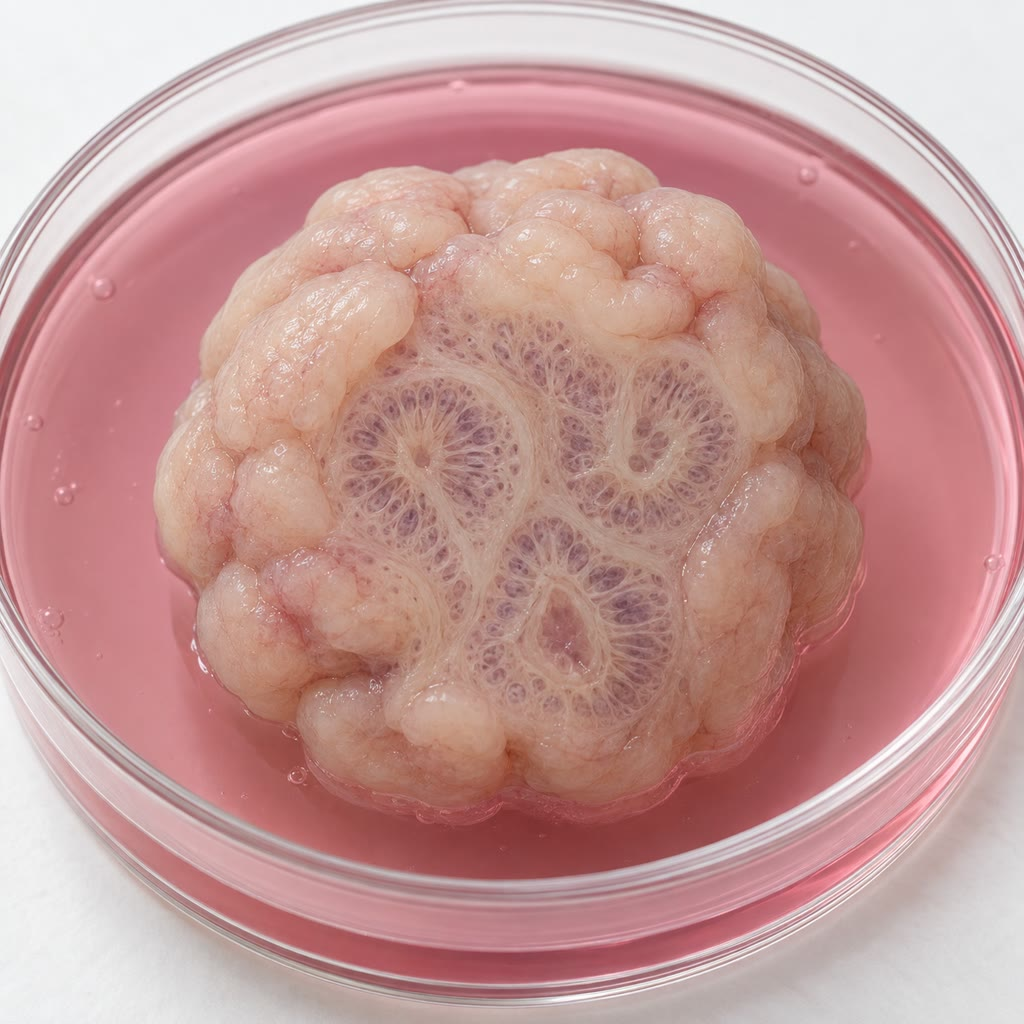
\includegraphics[width=0.4\linewidth]{images/book5/ai/b5-24-brain-organoid.jpg}\hspace{0.04\linewidth}
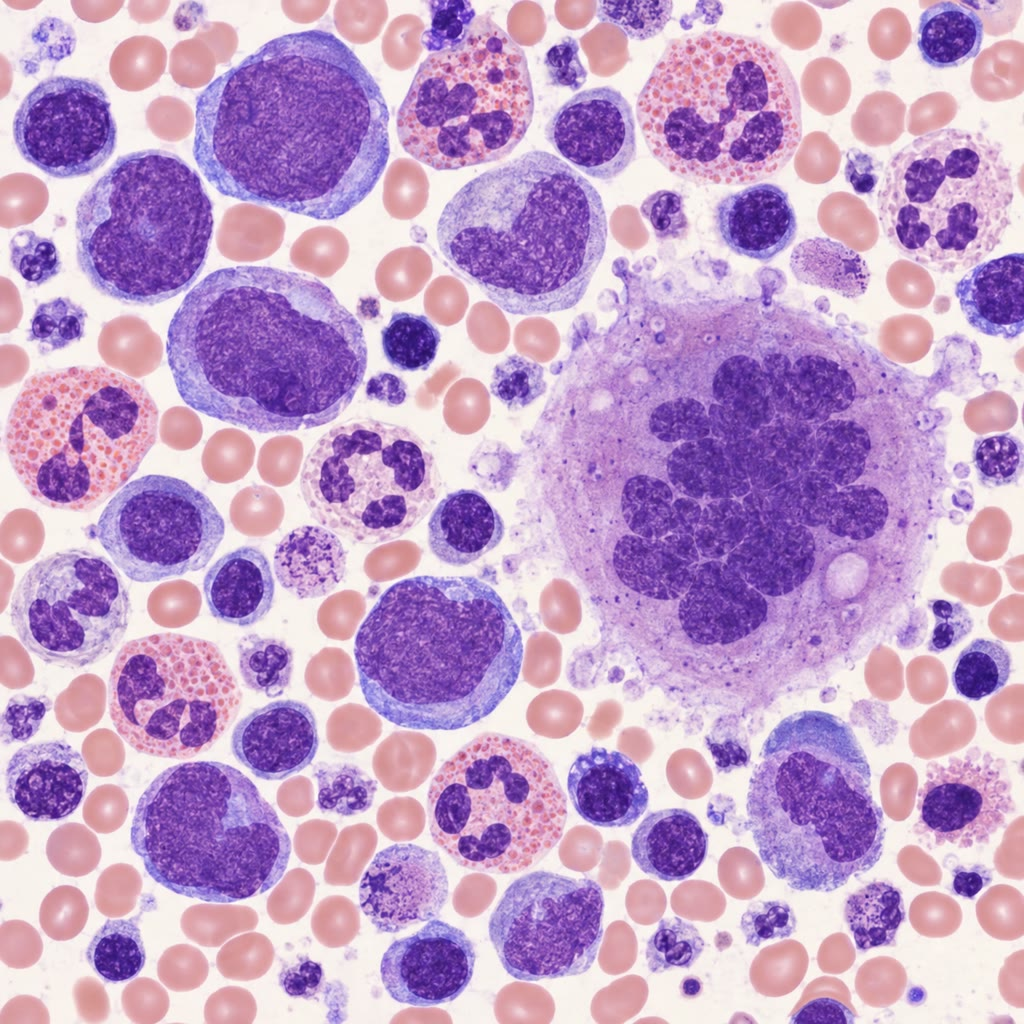
\includegraphics[width=0.4\linewidth]{images/book5/ai/b5-24-bone-marrow-smear.jpg}

{\small Left: a cerebral \omterm{def:b3:stem-cells:pluripotency}{organoid} grown from human pluripotent cells
--- a few millimetres of self-organised cortex-like tissue, with
ventricle-like cavities and layered neurons. Right: a bone-marrow
smear, the hierarchy of the first figure seen all at once: blasts,
maturing granulocytes, red-cell precursors and a megakaryocyte.}
\end{omfigure}

\begin{method}[Lineage tracing]\label{met:b3:stem-cells:tracing}
\index{lineage tracing}\index{Cre recombinase}
To find which cells are the \omterm{def:b3:stem-cells:stem}{stem cells} of a tissue: (1) choose a gene
expressed by the candidate cells and put under its promoter an
inducible recombinase (Cre-ER, active only when tamoxifen is given);
(2) in the same animal, a reporter gene that becomes permanently
active when the recombinase cuts a stop cassette out of it --- a
colour that is inherited by every descendant; (3) give one dose of
tamoxifen to mark the candidate cells at one moment; (4) harvest
tissue at intervals and score the marked clones: a clone that grows,
persists for months and contains every cell type of the tissue came
from a \omterm{def:b3:stem-cells:stem}{stem cell}; a clone that is shed within a week came from a
transit cell. (5) With a multicolour reporter, follow the competition
between clones. (6) Test function directly by killing the marked cells
with a toxin receptor expressed under the same promoter, and see
whether the tissue fails to renew.
\end{method}

\section{Regeneration}

\begin{definition}[How animals regrow]\label{def:b3:stem-cells:regeneration}
\index{regeneration}\index{neoblast}\index{blastema}\index{dedifferentiation}\index{compensatory growth}
Regeneration takes three routes. \emph{Hydra} and the planarian rely on
adult pluripotent \omterm{def:b3:stem-cells:stem}{stem cells}: a planarian's \emph{neoblasts}, a fifth
of its cells, are the only dividing cells it has, migrate to a wound,
and rebuild any missing part guided by positional signals (a Wnt
gradient tells the piece which end is the tail; block it and a tail
piece grows a second head). Salamanders rebuild a limb from a
\emph{blastema}, a cap of dividing cells at the stump formed largely by
\emph{dedifferentiation}: muscle fibres fragment into mononucleate
cells, cartilage and connective cells return to a \omterm{def:b3:stem-cells:stem}{progenitor} state,
each remembering its tissue of origin and its position along the limb,
and the blastema re-runs the embryonic limb programme under the wound
epidermis and the nerves, whose presence is required (denervate the
stump and nothing grows). Zebrafish regrow fins and heart the same
way, the heart's surviving muscle cells dividing to replace a fifth of
the ventricle in a month. Mammals do little of this: the liver regrows
its mass after two thirds is removed, but by the remaining cells
dividing in place (\emph{compensatory growth}), not by rebuilding the
lost lobes; a fingertip regenerates in children; the deer's antlers
grow anew each year from a stem-cell periosteum. Why not more is a
question of trade-offs: the mammalian wound response --- rapid clotting,
\omterm{def:b3:innate-immunity:inflammation}{inflammation}, fibroblast scar --- closes a wound fast against infection
and blood loss, and the scar forecloses the blastema; and cells that
can dedifferentiate and divide at will are cells that can become
\omterm{def:b3:cancer-biology:hallmarks}{cancers}, a risk a long-lived warm-blooded animal may not afford.
\end{definition}

\begin{omfigure}
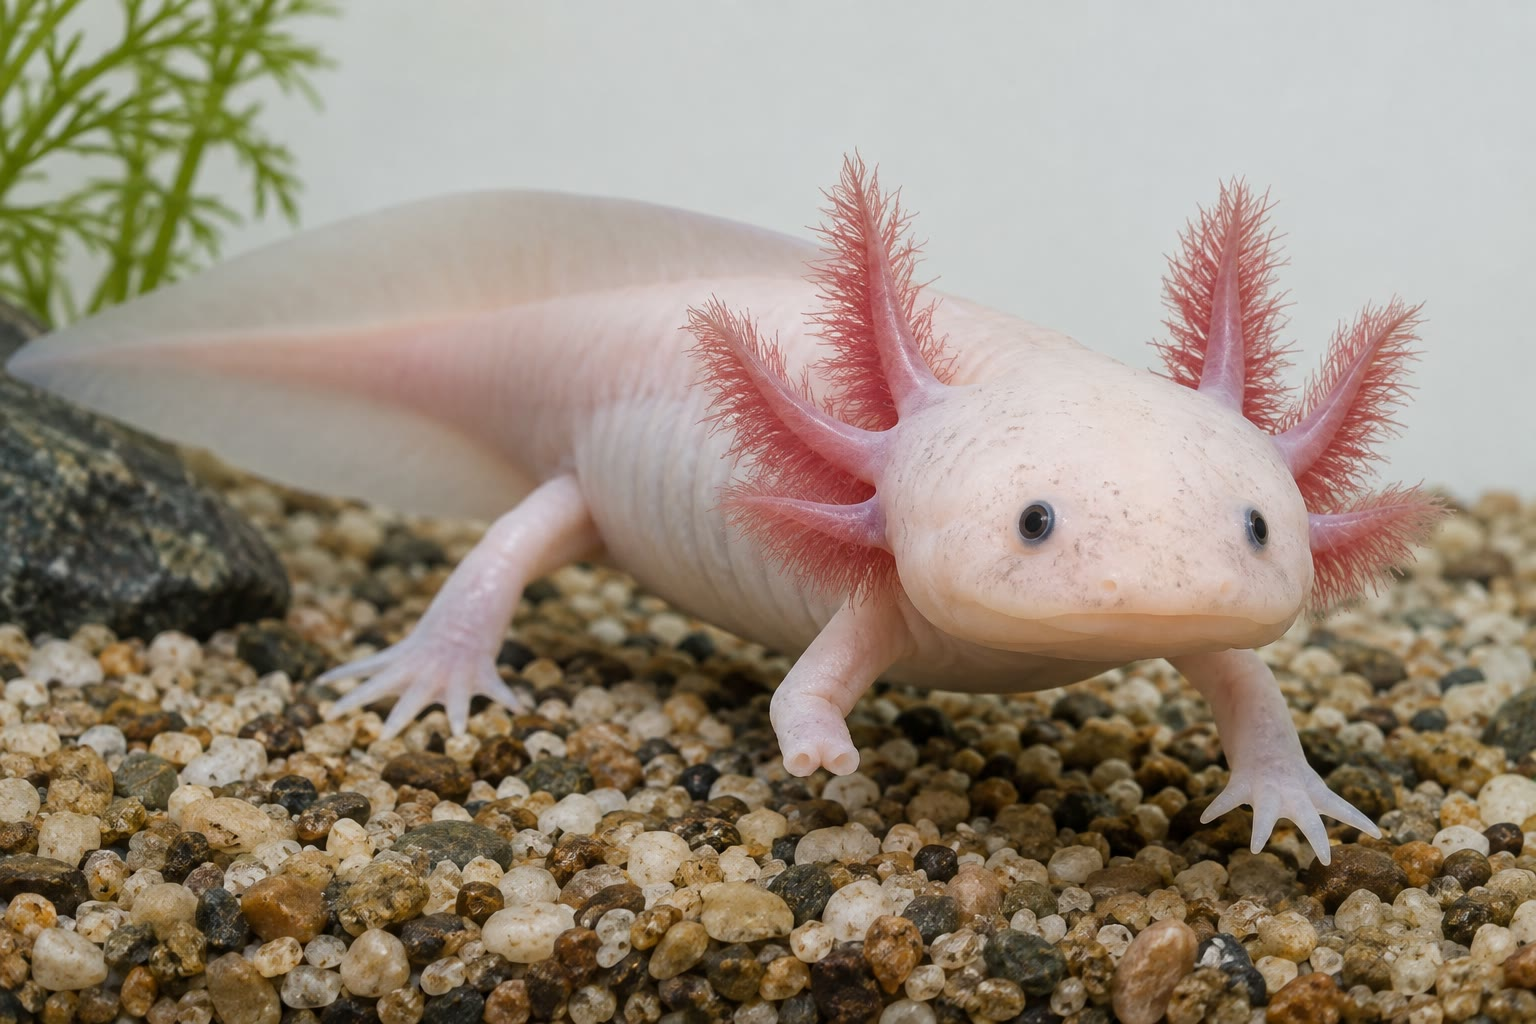
\includegraphics[width=0.46\linewidth]{images/book5/ai/b5-24-axolotl.jpg}\hspace{0.04\linewidth}
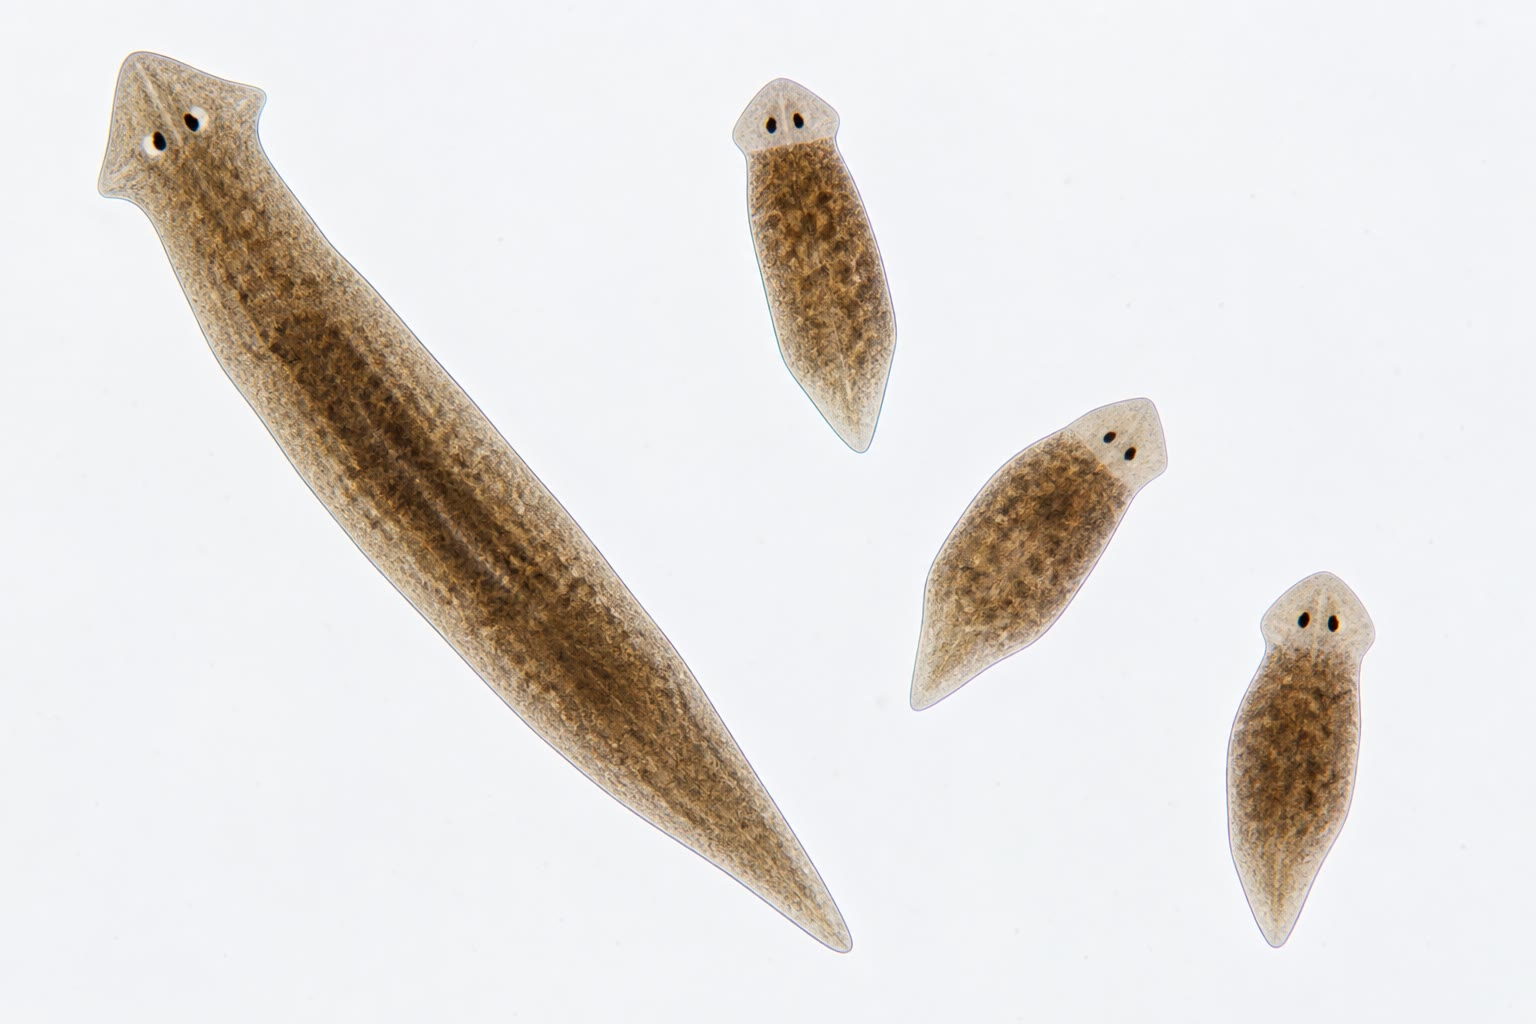
\includegraphics[width=0.46\linewidth]{images/book5/ai/b5-24-planarian-regeneration.jpg}

{\small Left: an axolotl, which regrows a limb in two months from a
\omterm{def:b3:stem-cells:regeneration}{blastema} of dedifferentiated cells and can do so all its life. Right: a
planarian cut into pieces, each piece regrowing a complete worm from its
\omterm{def:b3:stem-cells:regeneration}{neoblasts} within two weeks.}
\end{omfigure}

\begin{proof}[Evidence]
Morgan (1898) cut planarians into 279 pieces and found each regrew a
whole worm down to a limit of about a hundredth of the body; Reddien
and colleagues (2011) transplanted a single \omterm{def:b3:stem-cells:regeneration}{neoblast} into a lethally
irradiated worm and restored it entirely --- one cell, every tissue.
Kragl and colleagues (2009) made axolotls whose tissues were labelled
green one at a time and grafted them into unlabelled hosts: after
amputation, green muscle gave rise only to muscle, green cartilage to
cartilage --- the \omterm{def:b3:stem-cells:regeneration}{blastema} is not a pool of pluripotent cells but a
collection of lineage-restricted \omterm{def:b3:stem-cells:stem}{progenitors}, each dedifferentiated
only as far as its own tissue's \omterm{def:b3:stem-cells:stem}{progenitor}. Singer (1952) showed a
salamander limb regenerates only if a threshold number of nerve
fibres reaches the stump, and that rerouting a nerve to a wound on the
flank made a limb grow there.
\end{proof}

\section{The arithmetic of ageing}

\begin{theorem}[Telomeres and the Hayflick limit]\label{thm:b3:stem-cells:hayflick}
\index{telomere}\index{Hayflick limit}\index{end-replication problem}\index{telomerase}\index{replicative senescence}
Each chromosome ends in a \emph{telomere}, several kilobases of the
repeat TTAGGG. Because DNA polymerase cannot complete the lagging
strand's last stretch (the \emph{end-replication problem}), every
division shortens each telomere by $\Delta \approx$ \qtyrange{50}{100}{bp}.
Starting from $L_{0} \approx \qty{10}{kb}$ and triggering
\emph{\omterm{thm:b3:stem-cells:hayflick}{replicative senescence}} --- a permanent, p53-enforced arrest ---
when the shortest telomere reaches $L_{\text{crit}} \approx \qty{4}{kb}$,
a cell lineage can divide at most
\[
n_{\max} = \frac{L_{0} - L_{\text{crit}}}{\Delta} \approx \frac{6000}{50\text{--}100} \approx 60\text{--}120
\]
times: the \emph{\omterm{thm:b3:stem-cells:hayflick}{Hayflick limit}}, the fifty-odd population doublings
that human fibroblasts complete in culture before stopping. The
enzyme \emph{\omterm{def:b3:cancer-biology:telomerase}{telomerase}}, an RNA-templated reverse transcriptase,
re-extends the ends; it is active in the germ line, in embryonic and
many adult \omterm{def:b3:stem-cells:stem}{stem cells}, and in \qty{90}{\%} of \omterm{def:b3:cancer-biology:hallmarks}{cancers}, which have
escaped the limit by switching it back on. A \omterm{def:b3:stem-cells:stem}{stem cell} that divides
$d$ times a year with \omterm{def:b3:cancer-biology:telomerase}{telomerase} compensating a fraction $f$ of the
loss has $n_{\max} = (L_{0} - L_{\text{crit}})/[(1 - f)\Delta]$
divisions, and a lifetime of $n_{\max}/d$ years: with $f = 0.7$, $\Delta
= 60$, $d = 1$, some 330 years for a haematopoietic \omterm{def:b3:stem-cells:stem}{stem cell} --- but
its \omterm{def:b3:stem-cells:stem}{progenitors}, with \omterm{def:b3:cancer-biology:telomerase}{telomerase} off and twenty divisions to a red
cell, spend a fifth of their reserve at every lineage, which is why
old people's blood cells have shorter telomeres than young people's,
by about \qty{30}{bp} a year.
\end{theorem}
\begin{proof}
The loss per division is a fixed length, so telomere length falls
linearly with division number, $L_{n} = L_{0} - n\Delta$, and reaches
$L_{\text{crit}}$ at $n = (L_{0} - L_{\text{crit}})/\Delta$; with
partial compensation the net loss per division is $(1 - f)\Delta$.
Hayflick and Moorhead (1961) showed that normal human fibroblasts stop
after about fifty doublings whatever the culture conditions, that
cells frozen after twenty doublings and thawed complete only the
remaining thirty --- they count divisions, not time --- and that the
limit is lower for cells from old donors. Harley, Futcher and Greider
(1990) measured telomeres shortening with doublings in culture and with
donor age; Bodnar and colleagues (1998) put \omterm{def:b3:cancer-biology:telomerase}{telomerase} into normal
cells and they divided past the limit indefinitely without becoming
cancerous, which established the telomere as the clock.
\end{proof}

\begin{omfigure}
\begin{tikzpicture}
\begin{axis}[
  width=0.62\linewidth, height=5.4cm,
  axis x line=bottom, axis y line=left,
  xmin=0, xmax=120, ymin=0, ymax=11,
  xlabel={population doublings}, ylabel={telomere length (kb)},
  xlabel style={font=\small, at={(axis description cs:0.5,-0.12)}, anchor=north}, ylabel style={font=\small},
  tick label style={font=\small}, xtick={0,30,60,90,120}, ytick={4,7,10},
  clip=false,
]
\addplot[very thick, omDef, domain=0:60, samples=2] {10-0.1*x};
\addplot[very thick, omThm, domain=0:120, samples=2] {10-0.05*x};
\addplot[very thick, omMeth!70!black, domain=0:120, samples=2] {10-0.015*x};
\draw[dashed, gray] (axis cs:0,4) -- (axis cs:120,4); \node[font=\scriptsize, gray, anchor=north west] at (axis cs:2,3.9) {senescence at $L_{\text{crit}} = \qty{4}{kb}$};
\node[font=\scriptsize, omDef, anchor=south west] at (axis cs:63,4.3) {$\Delta = \qty{100}{bp}$: 60 doublings};
\node[font=\scriptsize, omThm, anchor=west] at (axis cs:70,8.0) {$\Delta = \qty{50}{bp}$: 120};
\node[font=\scriptsize, omMeth!70!black, anchor=south west, align=left] at (axis cs:78,9.3) {telomerase compensating\\\qty{70}{\%}: 400};
\fill[omDef] (axis cs:60,4) circle (2pt); \fill[omThm] (axis cs:120,4) circle (2pt);
\end{axis}
\end{tikzpicture}

{\small Telomeres as a division counter. A fixed loss per division gives
a straight line; where it crosses the critical length the lineage stops.
\omterm{def:b3:cancer-biology:telomerase}{Telomerase} flattens the slope and, fully active, abolishes the limit ---
in the germ line, and in \omterm{def:b3:cancer-biology:hallmarks}{cancers}.}
\end{omfigure}

\begin{proposition}[Gompertz's law]\label{prop:b3:stem-cells:gompertz}
\index{Gompertz law}\index{mortality rate}\index{hallmarks of ageing}\index{senescent cell}
Above about thirty the human death rate $\mu(t)$ --- the probability
of dying in the next year --- doubles every eight years: $\mu(t) =
\mu_{0}\,\mathrm{e}^{\gamma(t - t_{0})}$ with $\gamma = \ln 2/8 \approx
\qty{0.087}{yr^{-1}}$ (Gompertz, 1825). The survival to age $t$ is then
\[
S(t) = \exp\!\Bigl[-\frac{\mu_{0}}{\gamma}\bigl(\mathrm{e}^{\gamma(t - t_{0})} - 1\bigr)\Bigr],
\]
a curve flat for decades and then falling steeply, with a median
lifespan $t_{1/2} = t_{0} + \gamma^{-1}\ln(1 + \gamma\ln 2/\mu_{0})$:
for $\mu_{0} = 10^{-3}$ per year at thirty, about $30 + 47 = 77$ years.
The same law, with different constants, holds for mice (doubling time
three months), dogs, flies and worms: ageing is an exponential rise in
vulnerability, not a clock that stops. The biology behind the exponent
is a set of interacting \emph{hallmarks}: accumulated DNA damage and
epigenetic drift, telomere attrition, loss of proteostasis,
mitochondrial decline, exhaustion of stem-cell pools, the accumulation
of \emph{\omterm{prop:b3:stem-cells:gompertz}{senescent cells}} that no longer divide but secrete
inflammatory signals, and chronic \omterm{def:b3:innate-immunity:inflammation}{inflammation}; in mice, clearing
\omterm{prop:b3:stem-cells:gompertz}{senescent cells} or restricting calories extends life, and in worms a
single mutation in the insulin-like pathway doubles it. Whether the
exponent can be lowered in humans, rather than the constant $\mu_{0}$
which medicine has reduced tenfold in a century, is the open question.
\end{proposition}
\begin{proof}
If $\mu$ is the hazard, $\mathrm{d}S/\mathrm{d}t = -\mu(t)S$, so $\ln S =
-\int_{t_{0}}^{t}\mu = -(\mu_{0}/\gamma)(\mathrm{e}^{\gamma(t-t_{0})} -
1)$. Setting $S = 1/2$: $\mathrm{e}^{\gamma(t-t_{0})} = 1 + \gamma\ln 2/
\mu_{0}$, whence the median; with $\gamma = 0.087$ and $\mu_{0} =
10^{-3}$, $\ln(1 + 60) = 4.1$, $t - t_{0} = 47$. The empirical law is
Gompertz's fit to English life tables; that it describes so many
species with a shared form and species-specific constants is admitted
here as the summary of a century of demography.
\end{proof}

\begin{omfigure}
\begin{tikzpicture}
\begin{semilogyaxis}[
  width=0.5\linewidth, height=5.2cm,
  axis x line=bottom, axis y line=left,
  xmin=20, xmax=100, ymin=0.0003, ymax=1,
  xlabel={age (years)}, ylabel={death rate per year},
  xlabel style={font=\small, at={(axis description cs:0.5,-0.12)}, anchor=north}, ylabel style={font=\small},
  tick label style={font=\small}, xtick={30,50,70,90}, ytick={0.001,0.01,0.1,1}, yticklabels={0.001,0.01,0.1,1},
  clip=false,
]
\addplot[very thick, omDef, domain=30:100, samples=2] {0.001*exp(0.0866*(x-30))};
\node[font=\scriptsize, omDef, anchor=north west, align=left] at (axis cs:32,0.3) {$\mu = \mu_{0}\,\mathrm{e}^{\gamma(t-30)}$\\doubling every 8 years};
\end{semilogyaxis}
\begin{axis}[
  at={(0.55\linewidth,0)}, anchor=south west,
  width=0.43\linewidth, height=5.2cm,
  axis x line=bottom, axis y line=left,
  xmin=20, xmax=110, ymin=0, ymax=1.05,
  xlabel={age (years)}, ylabel={fraction surviving},
  xlabel style={font=\small, at={(axis description cs:0.5,-0.12)}, anchor=north}, ylabel style={font=\small},
  tick label style={font=\small}, xtick={30,50,77,100}, ytick={0.5,1},
  clip=false,
]
\addplot[very thick, omThm, domain=30:110, samples=80] {exp(-(0.001/0.0866)*(exp(0.0866*(x-30))-1))};
\draw[dashed, gray] (axis cs:77,0) -- (axis cs:77,0.5) -- (axis cs:20,0.5);
\node[font=\scriptsize, omThm, anchor=north east, align=right] at (axis cs:75,0.45) {median\\77 years};
\end{axis}
\end{tikzpicture}

{\small Gompertz's law. Left: on a logarithmic axis the death rate is a
straight line from thirty onward. Right: the survival curve that
follows --- a plateau, then a cliff, with the median where the hazard's
integral reaches $\ln 2$.}
\end{omfigure}

\begin{remark}[Renewal and its price]\label{rem:b3:stem-cells:remark}
A body that renews itself must keep cells that can divide
indefinitely, and cells that can divide indefinitely are the material
of \omterm{def:b3:cancer-biology:hallmarks}{cancer}; a body that guards against \omterm{def:b3:cancer-biology:hallmarks}{cancer} by counting divisions and
enforcing \omterm{def:b3:cell-cycle-apoptosis:other}{senescence} must, in time, run short of cells that can divide.
The stem-cell hierarchy is one solution --- few slow cells protected in
\omterm{def:b3:stem-cells:stem}{niches}, many fast cells that soon die --- and the \omterm{thm:b3:stem-cells:hayflick}{Hayflick limit} another,
and the exponential of Gompertz is the sum of their costs. The
salamander pays differently: it tolerates cells that dedifferentiate
and regrows a leg, and it is cold-blooded, slow and rarely lives long
enough to pay the \omterm{def:b3:cancer-biology:hallmarks}{cancer} bill. The cells you were born with are, for
the most part, not the cells you have; the ones that made the
replacements are the ones you have to keep.
\end{remark}

\section{Exercises}

\begin{exercise}[$\star$]\label{exo:b3:stem-cells:1}
Define \omterm{def:b3:stem-cells:stem}{self-renewal}, potency, \omterm{def:b3:stem-cells:stem}{niche} and \omterm{def:b3:stem-cells:stem}{transit-amplifying cell}, and
give an example of each in the gut.
\end{exercise}

\begin{exercise}[$\star$]\label{exo:b3:stem-cells:2}
What did the spleen-colony assay show, and which property of a \omterm{def:b3:stem-cells:stem}{stem
cell} required a second mouse to demonstrate?
\end{exercise}

\begin{exercise}[$\star$]\label{exo:b3:stem-cells:3}
Name the four Yamanaka factors and explain why \omterm{def:b3:stem-cells:pluripotency}{reprogramming} takes
weeks and succeeds in a thousandth of cells.
\end{exercise}

\begin{exercise}[$\star$]\label{exo:b3:stem-cells:4}
Contrast the planarian's and the salamander's routes to \omterm{def:b3:stem-cells:regeneration}{regeneration},
and say what Kragl's grafting experiments showed about the \omterm{def:b3:stem-cells:regeneration}{blastema}.
\end{exercise}

\begin{exercise}[$\star\star$]\label{exo:b3:stem-cells:5}
Telomeres start at \qty{11}{kb}, \omterm{def:b3:cell-cycle-apoptosis:other}{senescence} at \qty{5}{kb}, loss
\qty{75}{bp} per division. \omterm{thm:b3:stem-cells:hayflick}{Hayflick limit}? Cells from a 70-year-old
donor have \qty{8}{kb}: remaining doublings? If \omterm{def:b3:cancer-biology:telomerase}{telomerase} compensates
\qty{60}{\%} of the loss, limit?
\end{exercise}

\begin{exercise}[$\star\star$]\label{exo:b3:stem-cells:6}
A crypt holds 14 \omterm{def:b3:stem-cells:stem}{stem cells} dividing once a day, feeding transit cells
that divide 4 more times, and the crypt supplies \num{300} cells a day
to its villus. Check the arithmetic: how many stem-cell divisions a day
produce differentiating daughters, and how many \omterm{def:b3:stem-cells:stem}{stem cells}' worth of
divisions is that?
\end{exercise}

\begin{exercise}[$\star\star$]\label{exo:b3:stem-cells:7}
The body makes $2\times 10^{11}$ red cells a day, each the product of
about 20 divisions from a \omterm{def:b3:stem-cells:stem}{stem cell}. How many stem-cell divisions a day
does that require, and, with \num{10000} \omterm{def:b3:stem-cells:stem}{stem cells}, how often does each
divide? Compare with the observed ``about once a year'' and explain the
discrepancy.
\end{exercise}

\begin{exercise}[$\star\star$]\label{exo:b3:stem-cells:8}
With $\gamma = \qty{0.087}{yr^{-1}}$ and $\mu_{0} = 10^{-3}$ at thirty,
compute the death rate at 50, 70 and 90, the survival to 70 and 90, and
the median lifespan. What does halving $\mu_{0}$ do to the median? What
does halving $\gamma$ do?
\end{exercise}

\begin{exercise}[$\star\star$]\label{exo:b3:stem-cells:9}
Two thirds of a rat's liver is removed. The remaining hepatocytes, all
of which divide, restore the mass in ten days. How many divisions does
each need? Why is this called \omterm{def:b3:stem-cells:regeneration}{compensatory growth} and not \omterm{def:b3:stem-cells:regeneration}{regeneration},
and what does the liver \emph{not} rebuild?
\end{exercise}

\begin{exercise}[$\star\star\star$]\label{exo:b3:stem-cells:10}
\omterm{prop:b3:stem-cells:crypt}{Neutral drift}: $N$ \omterm{def:b3:stem-cells:stem}{stem cells} in a \omterm{def:b3:stem-cells:stem}{niche} divide symmetrically; at each
event one cell divides and one is lost at random, so the number of a
given clone performs a random walk between $0$ and $N$. Argue that the
probability a clone of $k$ cells eventually takes over the \omterm{def:b3:stem-cells:stem}{niche} is
$k/N$, and that with $N = 14$ a single-cell clone has a $1/14$ chance.
What does this predict for the fate of a \omterm{def:b3:stem-cells:stem}{stem cell} carrying a new
neutral mutation?
\end{exercise}

\begin{exercise}[$\star\star\star$]\label{exo:b3:stem-cells:11}
A mutation gives a stem-cell clone a \qty{10}{\%} advantage in the
competition of \cref{exo:b3:stem-cells:10}. Explain qualitatively why
its take-over probability rises well above $k/N$, why crypts and marrow
of old people are increasingly dominated by a few clones (clonal
haematopoiesis), and why this is a first step toward \omterm{def:b3:cancer-biology:hallmarks}{cancer} without
being \omterm{def:b3:cancer-biology:hallmarks}{cancer}.
\end{exercise}

\begin{exercise}[$\star\star\star$]\label{exo:b3:stem-cells:12}
Suppose the Gompertz exponent $\gamma$ reflects a rate of accumulating
damage and the constant $\mu_{0}$ the environment. Medicine has cut
$\mu_{0}$ tenfold since 1900 without changing $\gamma$. Compute the gain
in median lifespan that tenfold reduction gives, and the further gain
from another tenfold cut; explain why the returns diminish, and what a
\qty{20}{\%} cut in $\gamma$ would do instead.
\end{exercise}

\section{Problem: The Cells You Were Born With}

\begin{problem}[{Weekend problem --- a body's renewal in numbers: the
blood's hierarchy and what it asks of its stem cells, the crypt's
drift, the telomere clock and how telomerase and progenitors spend it,
the Gompertz curve of the population, and the trade-offs a regenerating
animal accepts, ending on the Hayflick count, the stem cell's lifetime
reserve and the median lifespan}]
\label{pb:b3:stem-cells:1}
Data: red cells $2.5\times 10^{11}$ a day, granulocytes $10^{11}$ a
day; $20$ divisions from \omterm{def:b3:stem-cells:stem}{stem cell} to mature cell; \num{10000}
haematopoietic \omterm{def:b3:stem-cells:stem}{stem cells}. Telomeres: $L_{0} = \qty{10}{kb}$,
$L_{\text{crit}} = \qty{4}{kb}$, $\Delta = \qty{60}{bp}$ per division;
\omterm{def:b3:cancer-biology:telomerase}{telomerase} in \omterm{def:b3:stem-cells:stem}{stem cells} compensates $f = 0.7$; none in \omterm{def:b3:stem-cells:stem}{progenitors}.
Crypt: $N = 14$ \omterm{def:b3:stem-cells:stem}{stem cells}, one division a day. Gompertz: $\mu_{0} =
10^{-3}$ per year at age 30, $\gamma = \qty{0.087}{yr^{-1}}$. Axolotl
limb: \qty{40}{mm} regrown in \qty{60}{days}; \omterm{def:b3:stem-cells:regeneration}{blastema} $10^{5}$ cells
growing to $10^{8}$.

\medskip
\noindent\textbf{Part I --- The blood.}
\begin{enumerate}
  \item Cells produced per day in total, and per second.
  \item Each mature cell is the end of $20$ divisions: how many cells
        result from one committed daughter of a \omterm{def:b3:stem-cells:stem}{stem cell}? How many
        committed daughters a day are needed?
  \item With \num{10000} \omterm{def:b3:stem-cells:stem}{stem cells}, how many differentiating divisions
        per \omterm{def:b3:stem-cells:stem}{stem cell} per day does that imply? Per year?
  \item Measured stem-cell division is about once a year. Reconcile:
        what must the \omterm{def:b3:stem-cells:stem}{progenitors} do that the calculation of
        question~3 assumed the \omterm{def:b3:stem-cells:stem}{stem cells} did?
  \item \omterm{def:b3:stem-cells:stem}{Progenitors} have no \omterm{def:b3:cancer-biology:telomerase}{telomerase}. From \qty{10}{kb}, what telomere
        length does a red cell precursor reach after its $20$ divisions?
        Does it matter that it is above $L_{\text{crit}}$?
  \item A \omterm{def:b3:stem-cells:stem}{stem cell} dividing once a year with $f = 0.7$: net loss per
        division, divisions to \omterm{def:b3:cell-cycle-apoptosis:other}{senescence}, and years. Comment.
\end{enumerate}

\medskip
\noindent\textbf{Part II --- The crypt.}
\begin{enumerate}[resume]
  \item Divisions per crypt per day at the stem-cell tier; if half the
        events replace a lost \omterm{def:b3:stem-cells:stem}{stem cell} and half feed the transit zone,
        how many committed cells a day, and how many villus cells after
        $4$ transit divisions?
  \item A single-cell clone's take-over probability is $1/N$. Expected
        time to monoclonality is of order $N^{2}$ division events per
        cell; estimate it in days and compare with the confetti
        observations (months).
  \item A \omterm{def:b3:stem-cells:stem}{stem cell} acquires a mutation. Probability it is eventually
        fixed in its crypt? In how many of the $10^{7}$ crypts of a
        colon would a mutation arising once per crypt become fixed?
  \item Why does a crypt's drift protect against \omterm{def:b3:cancer-biology:hallmarks}{cancer} more than a
        tissue in which every \omterm{def:b3:stem-cells:stem}{stem cell} divides asymmetrically for life?
  \item After irradiation kills the \omterm{def:b3:stem-cells:stem}{stem cells}, transit cells revert
        and refill the \omterm{def:b3:stem-cells:stem}{niche}. What does this say about where stemness
        lives?
  \item Sketch the lineage-tracing experiment that distinguishes
        symmetric drift from \omterm{def:b3:stem-cells:stem}{asymmetric division}, and the two outcomes.
\end{enumerate}

\medskip
\noindent\textbf{Part III --- The clock.}
\begin{enumerate}[resume]
  \item \omterm{thm:b3:stem-cells:hayflick}{Hayflick limit} for a somatic lineage without \omterm{def:b3:cancer-biology:telomerase}{telomerase}.
  \item A fibroblast culture is frozen after $25$ doublings and thawed
        a decade later: doublings left? What does this show about what
        the cell counts?
  \item Leukocyte telomeres shorten by \qty{30}{bp} a year in adults.
        Starting from \qty{8}{kb} at twenty, when would they reach
        $L_{\text{crit}}$? Compare with lifespan and comment.
  \item \omterm{def:b3:cancer-biology:telomerase}{Telomerase} added to normal fibroblasts lets them pass the limit
        without becoming cancerous. \omterm{def:b3:cancer-biology:telomerase}{Telomerase} is active in \qty{90}{\%}
        of \omterm{def:b3:cancer-biology:hallmarks}{cancers}. Reconcile the two statements.
  \item Compute the Gompertz death rate at 40, 60, 80 and 100, and the
        survival to each.
  \item Median lifespan; and the age at which \qty{10}{\%} survive.
\end{enumerate}

\medskip
\noindent\textbf{Part IV --- Regrowing.}
\begin{enumerate}[resume]
  \item Axolotl: mean regrowth rate in mm/day; doublings for the
        \omterm{def:b3:stem-cells:regeneration}{blastema} to grow from $10^{5}$ to $10^{8}$ cells, and the mean
        doubling time over 60 days.
  \item If dedifferentiated cells divide like the \omterm{def:b3:stem-cells:regeneration}{blastema}'s throughout
        life and a division carries a $10^{-9}$ chance per cell of an
        oncogenic mutation, how many such mutations arise in one
        \omterm{def:b3:stem-cells:regeneration}{regeneration}? Why is the axolotl nonetheless almost never
        cancerous, and why might a mammal not get away with it?
  \item Denervating the stump stops \omterm{def:b3:stem-cells:regeneration}{regeneration}. Propose an experiment
        to show the nerve supplies a diffusible factor, and one
        possible identity of the factor.
  \item A planarian tail piece grows a second tail instead of a head
        when a Wnt inhibitor is knocked down. Explain with a gradient
        and the positional memory of the piece.
  \item Human liver after a two-thirds resection: fraction of
        hepatocytes that must divide once, twice, to restore the mass.
        Why is the result a working liver but the wrong shape?
  \item Why would a body that regenerated like an axolotl have a
        different Gompertz curve, and in which direction?
  \item Summarise: the Hayflick count (question~13), a telomerase-aided
        \omterm{def:b3:stem-cells:stem}{stem cell}'s divisions and years (question~6), and the median
        lifespan (question~18).
\end{enumerate}
\end{problem}
